\documentclass[10pt]{IEEEtran}

\title{Applying The SURF Algorithm to the Prokudin-Gorskii Image Set}
\author{Jeffrey-David Kapp, Sebastian Lenartowicz, and Vincent Yong}

\usepackage{listings}
\usepackage{color}
\usepackage{graphicx}
\usepackage{subfig}

% Colours for Python syntax highlighting (doesn't work out of the box)
\definecolor{deepblue}{rgb}{0,0,0.5}
\definecolor{deepred}{rgb}{0.6,0,0}
\definecolor{deepgreen}{rgb}{0,0.5,0}

\lstset{
	language=Python,
	basicstyle=\footnotesize\ttfamily,
	keywordstyle=\color{deepblue},
	stringstyle=\color{deepred},
	commentstyle=\color{deepgreen},
	showstringspaces=false
}

\newcommand{\composite}[1]{
	\centering
	\subfloat[``Raw'' composite.]{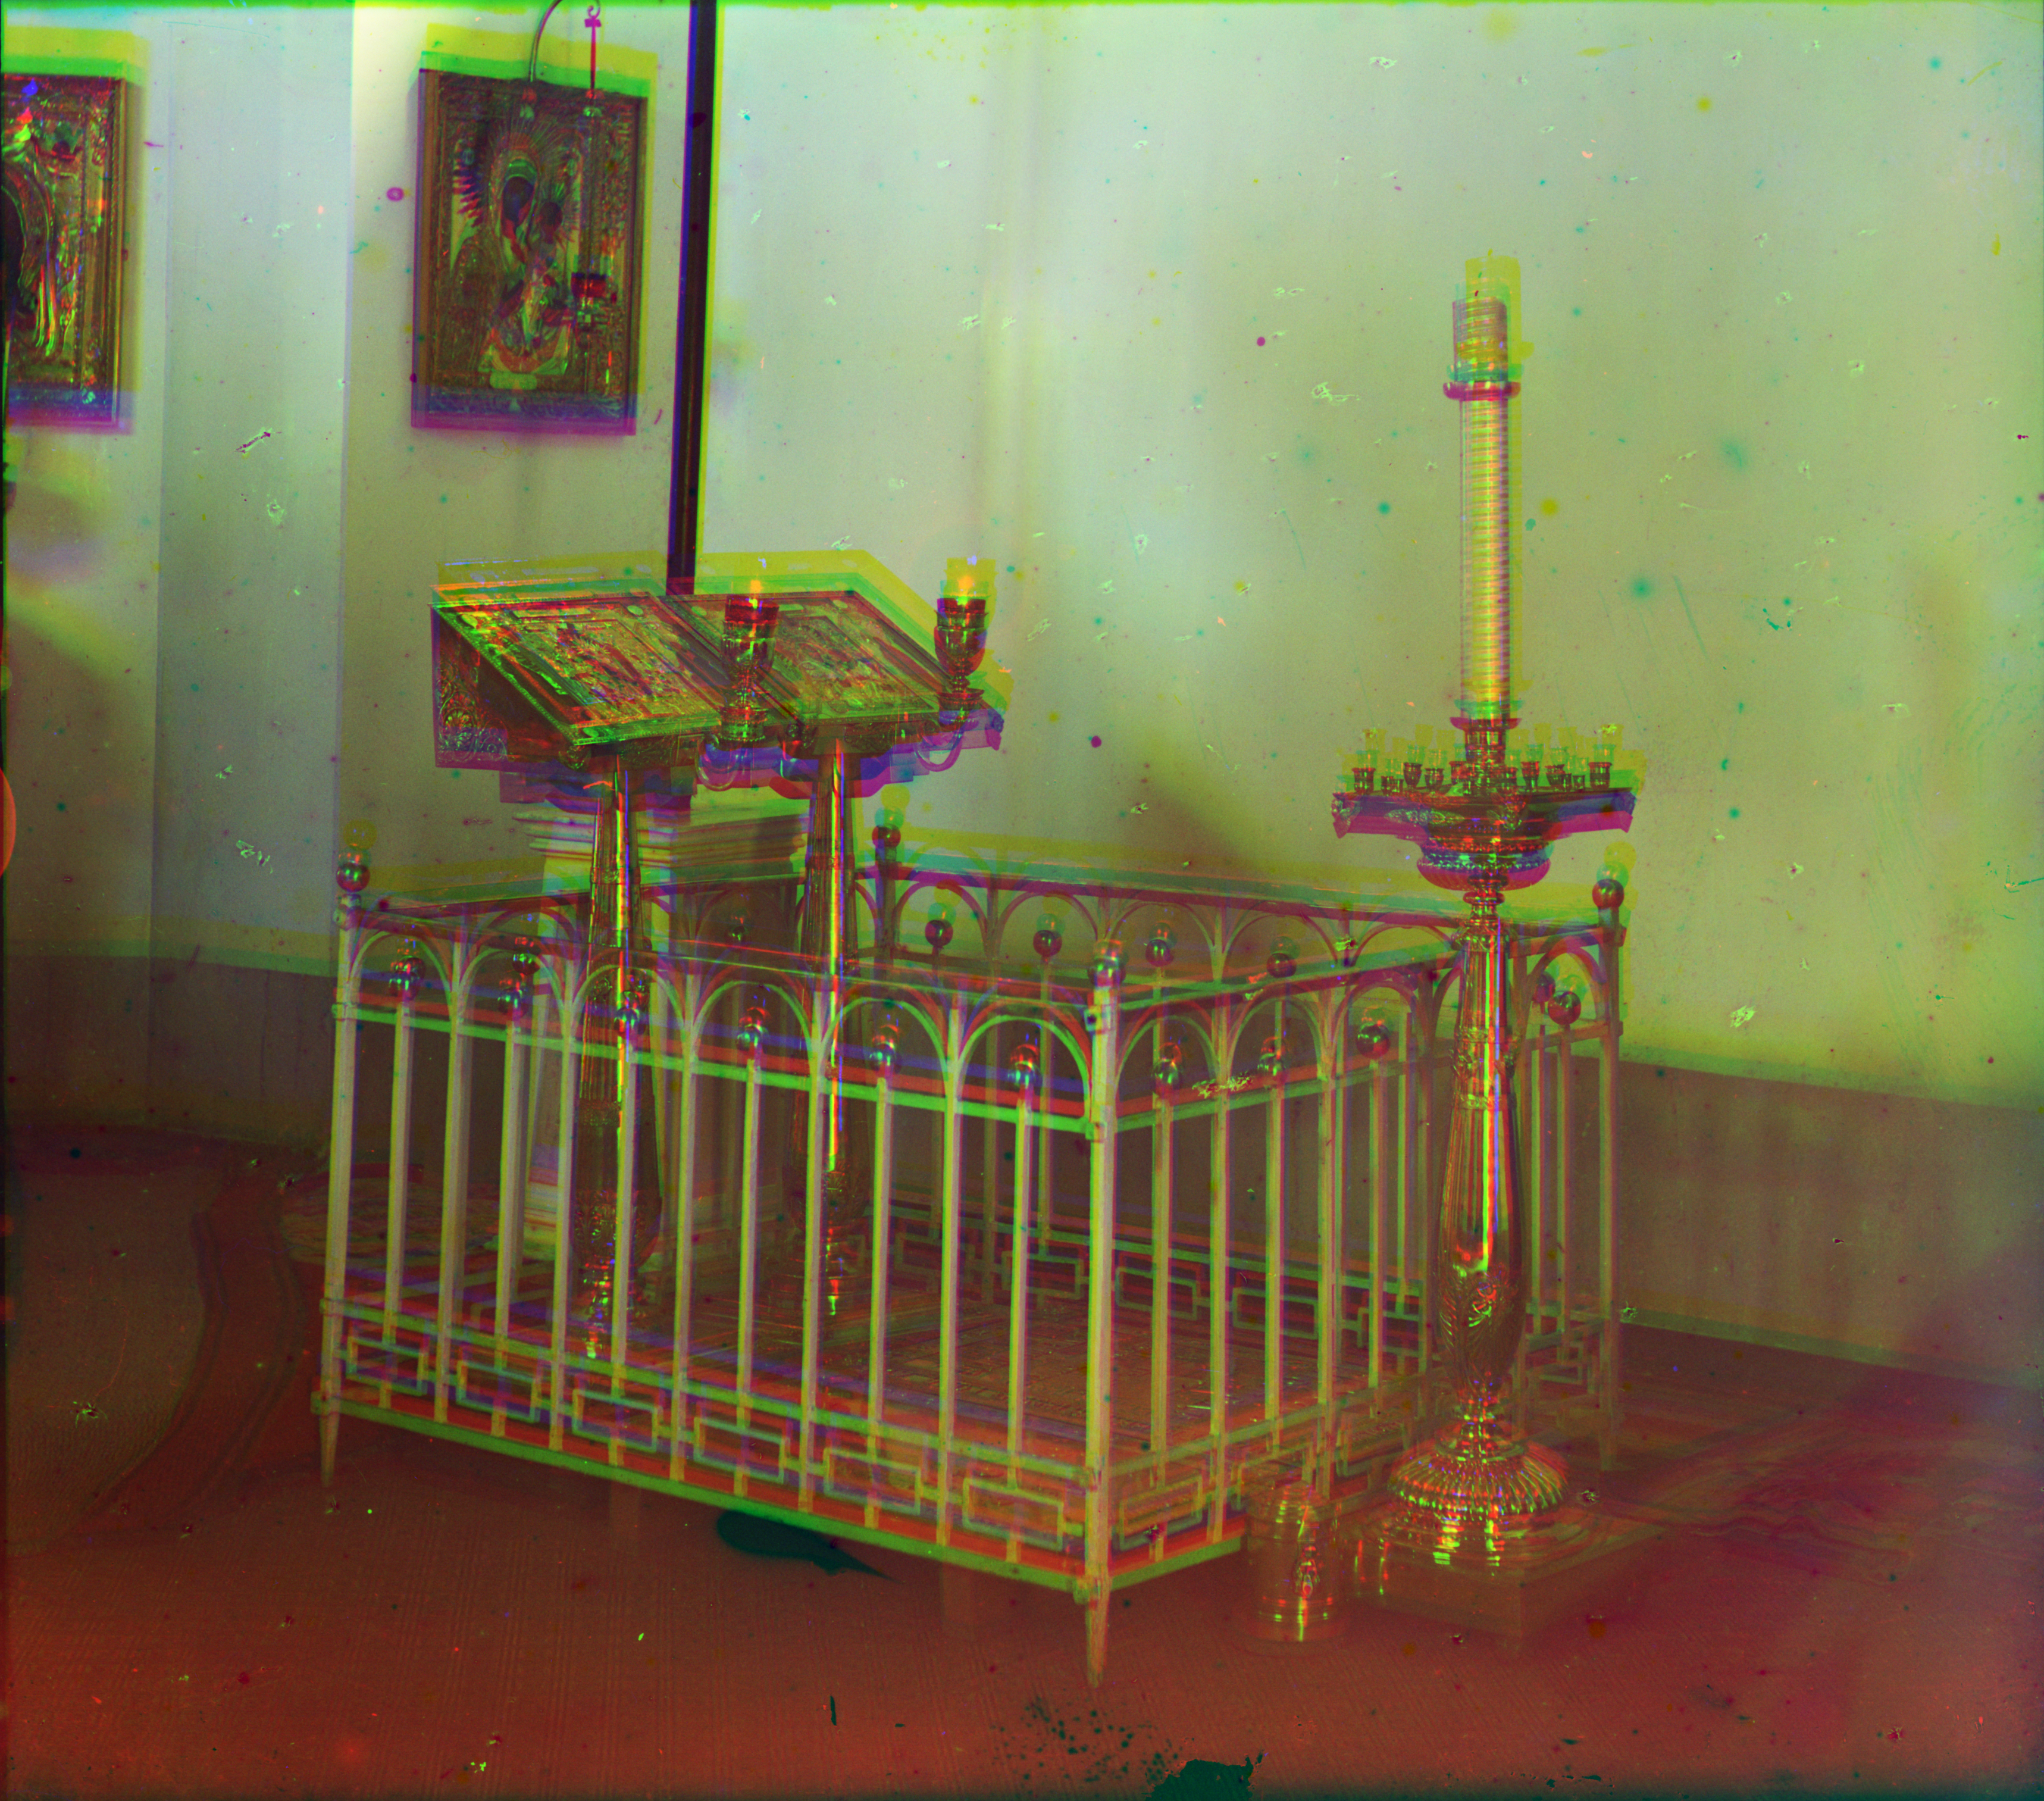
\includegraphics[width=0.45\textwidth]{../#1/original.png}}
	\hspace{0.05\textwidth}
	\subfloat[Composited image.]{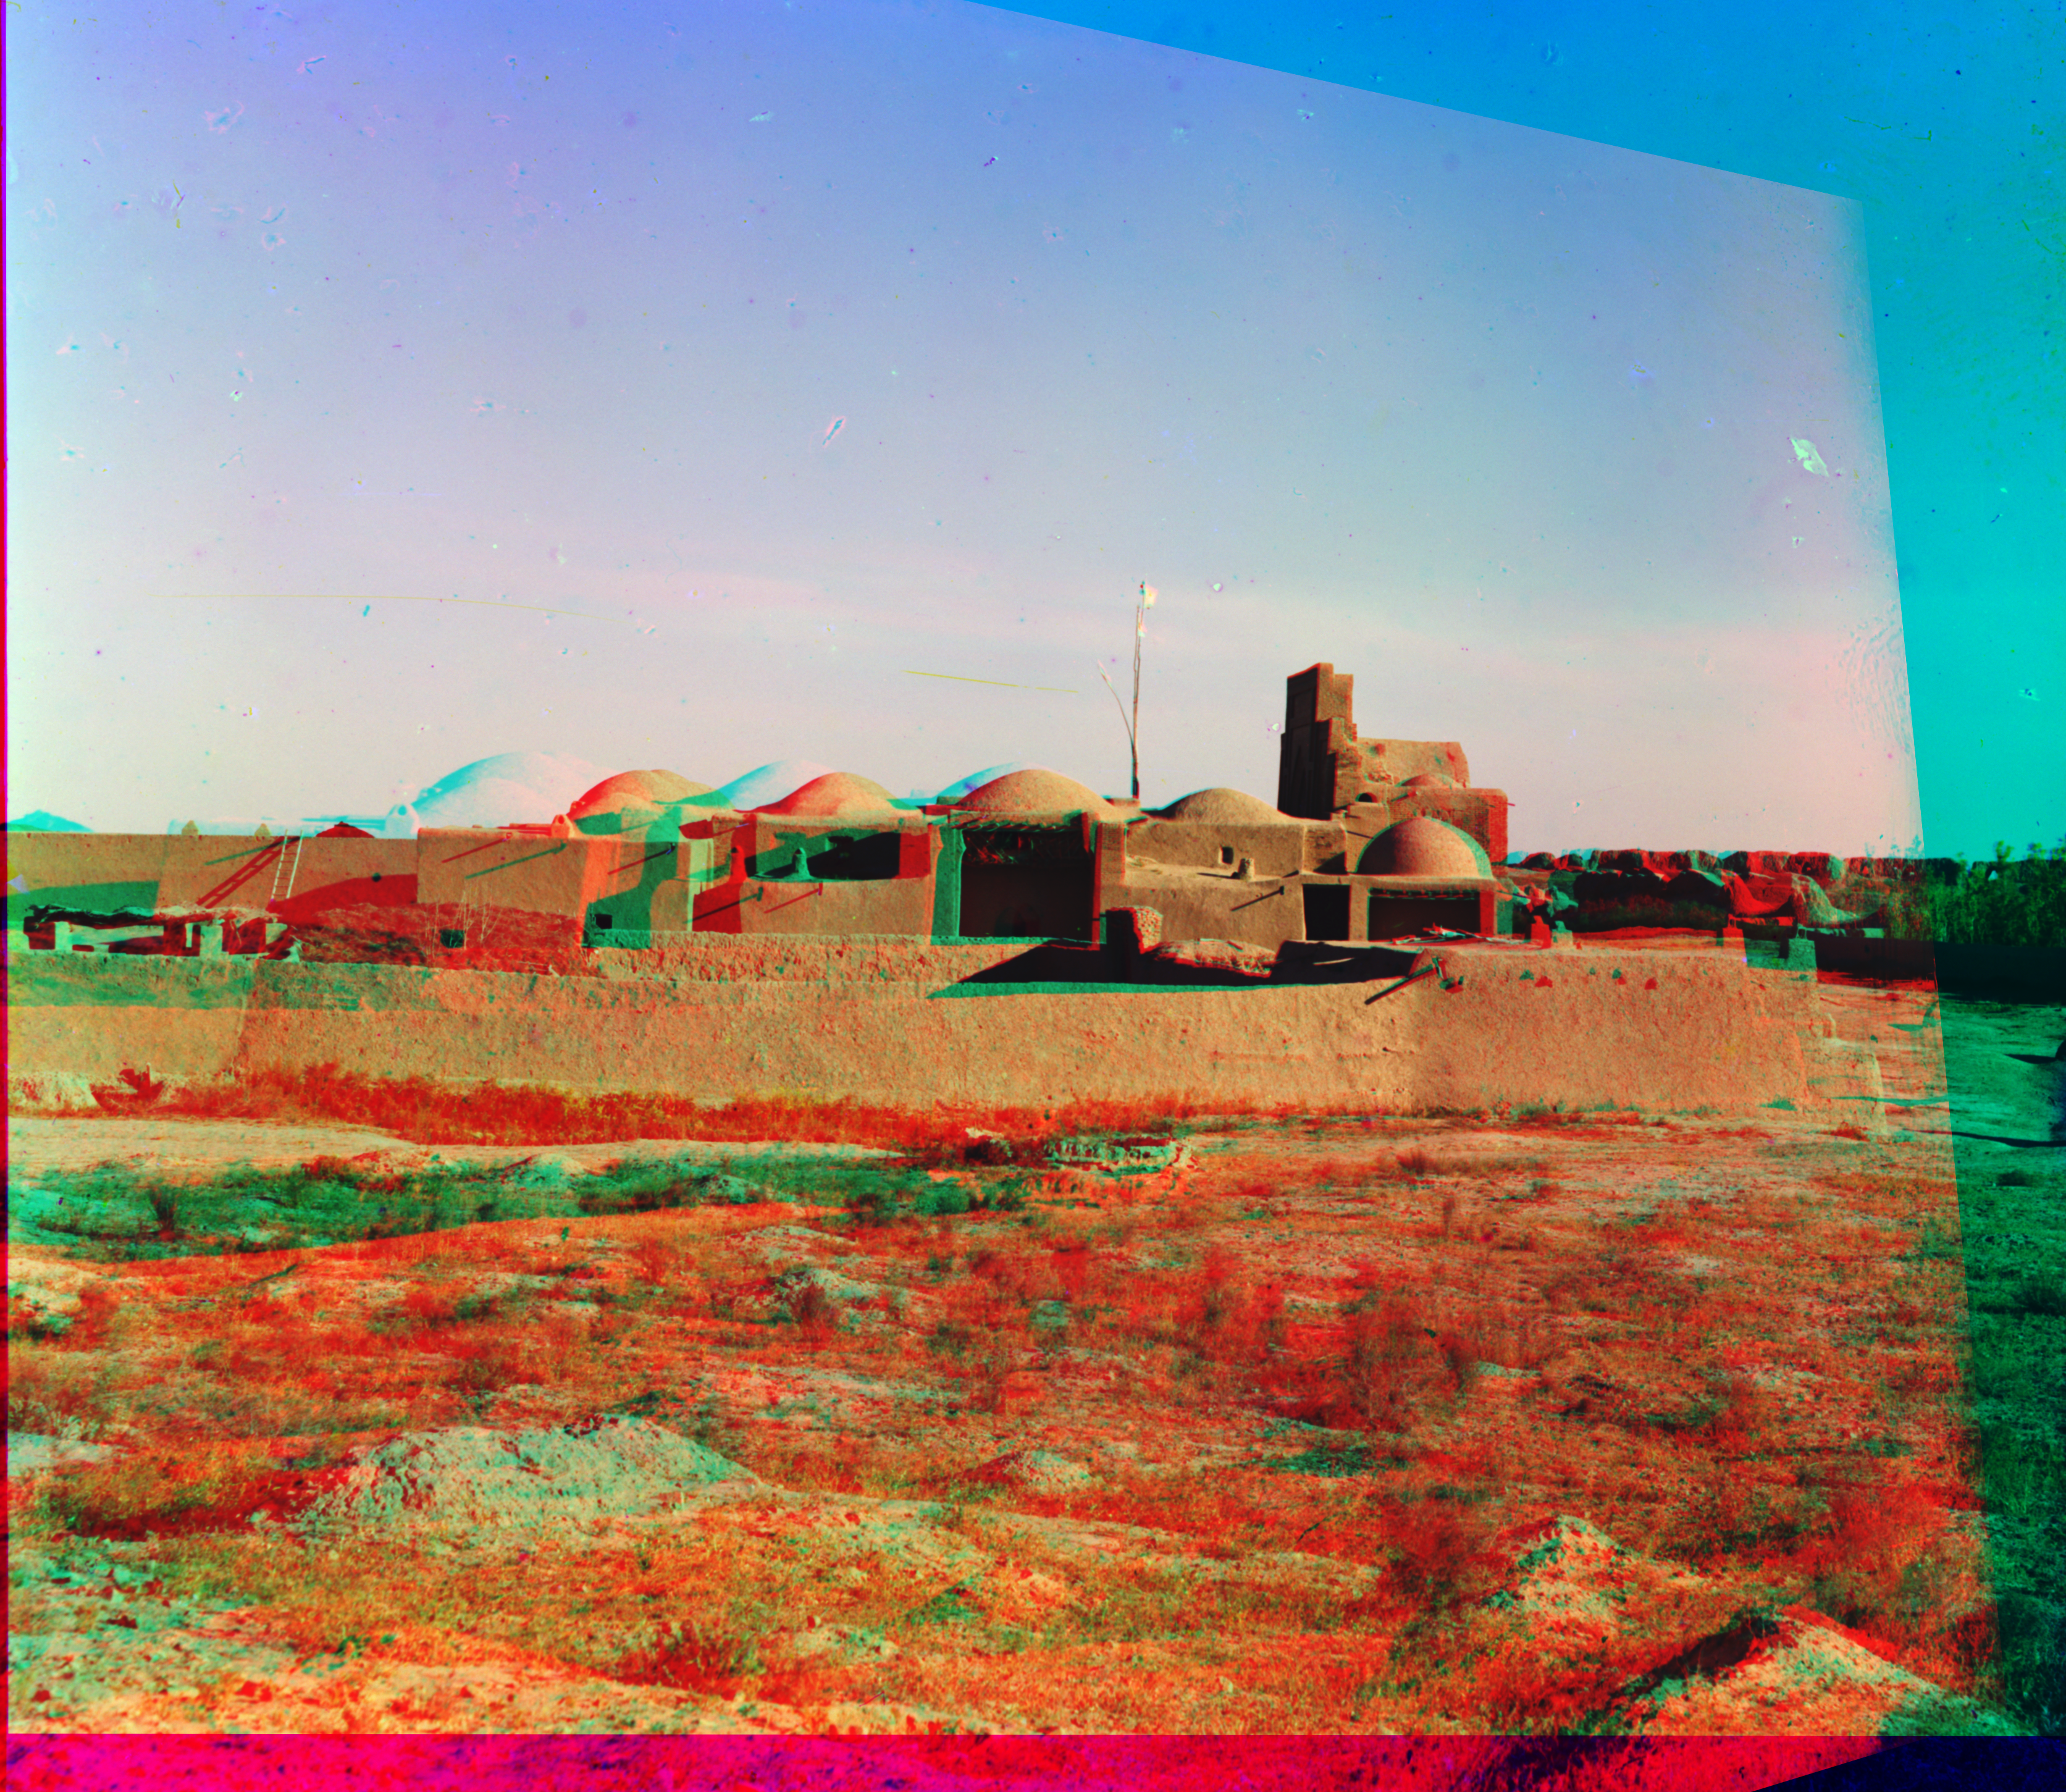
\includegraphics[width=0.45\textwidth]{../#1/composite.png}}
}

\begin{document}
\maketitle

	\section{Introduction}
	Since their rediscovery in 1948, the Prokudin-Gorskii images have attracted considerable academic attention for a variety of reasons. In computer science, this interest most often takes the form of testing image-registration and compositing algorithms \cite{minachin2007reconstruction} due to their unique structure; each image consists of three greyscales, which correspond to the three RGB channels. Though nominally centered on the same subject and aligned to each other, the image sets have slight but noticeable misalignment, which renders na\"ive compositing worthless -- the resultant image from simple compositing resembles the input to R/B 3D glasses more so than it does an actual colour photograph. By applying image-registration algorithms -- typically used in GIS and other areas where image mosaicking is a common activity -- it becomes possible to quickly and effectively composite these images and reveal the stunning colours of Imperial Russia. In order to do this, we apply the Speeded Up Robust Features (SURF) algorithm \cite{bay2006surf}, which is specifically designed for image pairs in which brightness values for the same objects may vary considerably.

	\section{Compositing the Images}
		Our image compositor, at its core, relies upon the OpenCV implementation of the SURF algorithm. It begins by loading each channel from a separate file, then using the red channel as a ``baseline'' from which to do SURF comparisons. The green and blue channels are both compared against the red, and the resultant keypoints matched against each other. If there is a difference in their position of less than 10\% of the image size, they are considered to be acceptable. Following this, the keypoints are used to find a homography (set of transformations) between the blue/green channels and the red channels. The transformations are then applied, and the resulting images composited onto each other to yield the final output. The full source code for the compositor can be found in Figure \ref{fig:code}.

	\section{Experiments}
		In order to test this approach, we selected 65 images from the Library of Congress' digitized collection. Each image was downloaded, and the three colour channels were manually cropped from the single file provided by the Library. These three files were then provided as input to the compositor, with the output being both a ``raw'' (unaligned) composite and the automatically aligned image.

		Of the 65 images tested, three failed to composite correctly and a fourth composited mostly correctly. In this case, a failure to composite refers to an image in which one or more channels are misaligned or distorted relative to the others, and a partial failure refers to an image in which the primary subject(s) are aligned correctly but some portion of the image is not.

		Due to the need for a manual cropping process, large colour bars, where the greyscale channel images do not quite overlap, appear in most of the composited images. These can be eliminated by better cropping or automatic segmentation.

	\section{Conclusions}
		Though the power of SURF in automatically aligning Prokudin-Gorskii images is clear, its limitations are clear as well. Because SURF often identifies keypoints that do not correspond to each other, it is necessary to employ some form of filtering -- often distance-based. In general, however, SURF was successful at compositing the images, and, with some form of adaptive thresholding parameter, could likely successfully align the failed images as well.

	\bibliographystyle{IEEEtran}
	\bibliography{IEEEabrv,references}

		\begin{figure*}
			\lstinputlisting{../surf.py}
			\caption{Source code for the image compositor.}
			\label{fig:code}
		\end{figure*}

\newpage

\begin{figure*}
	\composite{00010a}

	\caption{Image 00010a: The Camel. In this image, the compositor succeeded in correctly aligning the three channels. The small amount of colour ``ghosting'' around the middle of the camel's neck is likely a result of it having moved while having its photo taken.}
\end{figure*}

\begin{figure*}
	\composite{00011a}

	\caption{Image 00011a: Camel with Handler. Here again, the compositor succeeded in aligning the three channels. Some ghosting is visible around the camel's ears due to the difficulty in making an animal remain completely still. Additionally, the image has suffered some degradation, resulting in the large bright spot on the bag on the camel's back.}
\end{figure*}

\begin{figure*}
	\composite{00031a}

	\caption{Image 00031a: Church Candle Holder. Though the crop was inadvertently nearly perfect, some mismatching is still visible. The compositor was able to address this quite neatly. This image has suffered significant degradation at the upper and lower left corners, and subtle vignetting at the top.}
\end{figure*}

\begin{figure*}
	\composite{00111a}

	\caption{Image 00111a: The Ruin. Though only slightly misaligned, the compositor was nonetheless able to elicit improvement and align the channels perfectly. Some image degradation is evident along the right edge.}
\end{figure*}

\begin{figure*}
	\composite{00152a}

	\caption{Image 00152a: Alim Khan, Emir of Bukhara. This image is noteworthy in that, if the compositor is re-run with the distance parameter set to 25\%, there is significant distortion, resulting in a failed composite. Decreasing the threshold to 10\% results in the composite seen here.}
\end{figure*}

\begin{figure*}
	\composite{00223a}

	\caption{Image 00223a: The Windmill. The only example of a partial failure in our experiments -- though the field and building were aligned correctly, the red channel was somewhat distorted in the upper left corner. It is also evident that the glass negative was smashed at some point in its existence.}
\end{figure*}

\begin{figure*}
	\composite{00026a}

	\caption{Image 00026a: The Wooden Saints. One of three complete failures in our image set, in which the red channel became significantly distorted compared to the green and blue. Though this image composites correctly when the distance threshold is set to 25\%, this causes other images to fail.}
\end{figure*}

\begin{figure*}
	\composite{00384a}

	\caption{Image 00384a: The Reliquary. Like 00026a, this image fails to composite correctly. Unlike 00026a, however, it also fails when the threshold is set to 25\% -- this image, in fact, represents an improvement in performance vs. the 25\% threshold composite.}
\end{figure*}
\end{document}
